\subsection{Overview of Examples}
In this section, we establish some fundamental properties of solutions to the SIP under different QoI maps, as they relate to the skewness of the $Q$'s being compared.
We seek an estimated probability measure $\hat{\PP}_\pspace$ on the parameter space to converge (with respect to the metric $d_\text{TV}$) to some reference measure $\PP_\pspace$ as more samples (i.e., model evaluations), $\nsamps$ are used.
Such a reference measure could be either some known distribution taken as truth, or another approximation deemed to be sufficiently resolved for the given application or computational budget (i.e. higher-fidelity model, mesh, or Monte-Carlo sample-size).\footnote{However, we could also choose to interrogate the push-forward measures given by propagating the $\hat{\PP}_\pspace$ and $\PP_\pspace$ forward to a data space by a QoI map and taking the distance on the resulting output space.
This would measure the ability of the maps to reconstruct the output probability measure.}

In Figure~\ref{fig:voronoi_sols}, we illustrate the solution to the problem of comparing measures defined on two different (implicitly-defined) $\sa$s shown in Figure~\ref{fig:voronoi_issues}.
By introducing a third set against which both sample sets of size $\nsamps=50$, are compared, we can leverage theoretical results from Lemma~\ref{lem:measuresets} to rigorously compare solutions to the SIP under different maps.

\begin{figure}[ht]
\centering
	\begin{minipage}{.275\textwidth}
		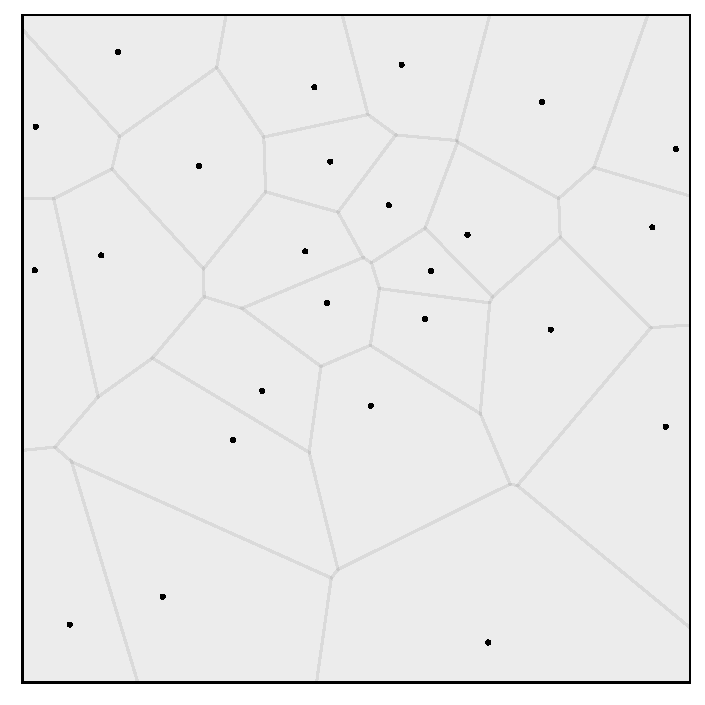
\includegraphics[width=\linewidth]{./images/voronoi_diagrams/voronoi_diagram_N25_r0_no_label}
	\end{minipage}
	\begin{minipage}{.4\textwidth}
		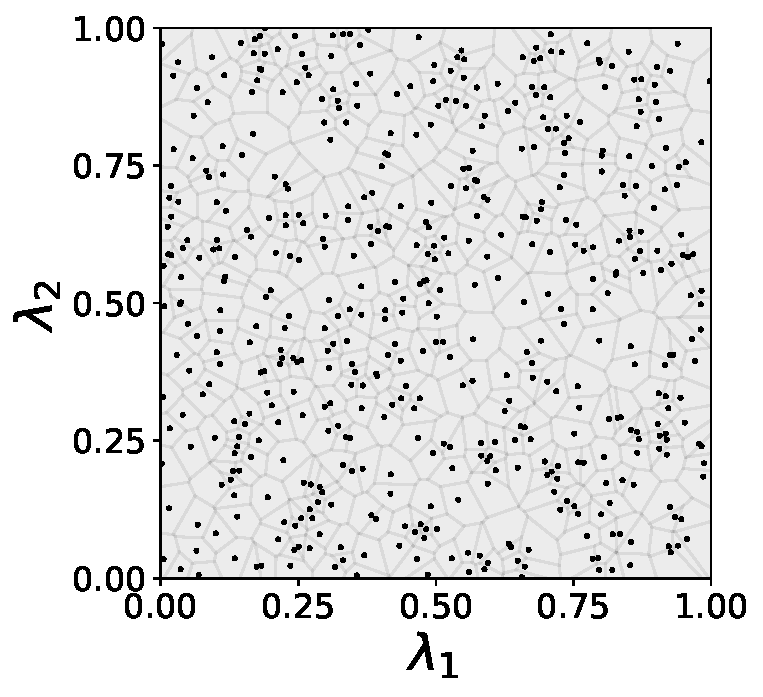
\includegraphics[width=\linewidth]{./images/voronoi_diagrams/voronoi_diagram_N500_r50}
	\end{minipage}
		\begin{minipage}{.275\textwidth}
		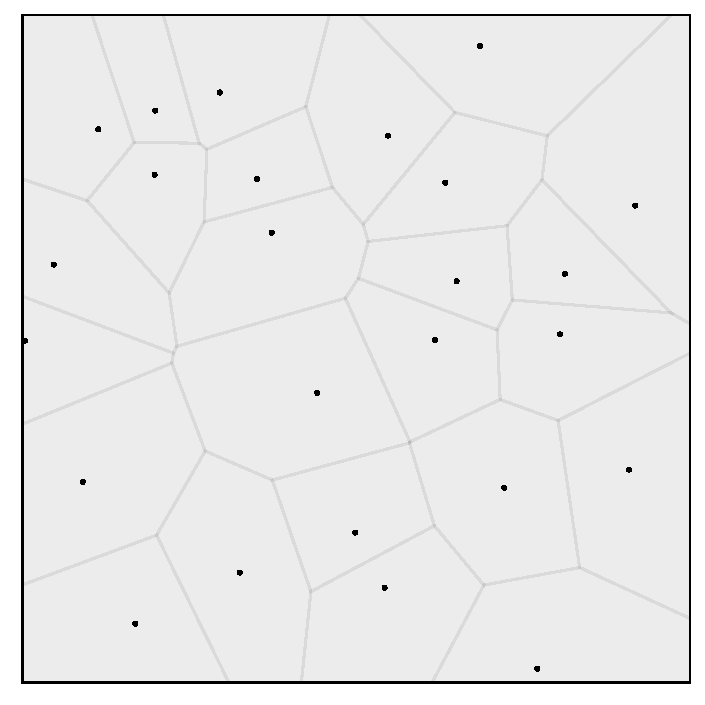
\includegraphics[width=\linewidth]{./images/voronoi_diagrams/voronoi_diagram_N25_r10_no_label}
	\end{minipage}
\caption{
(Left/Right): The two partitions from Figure~\ref{fig:voronoi_issues} will be projected onto a third reference partition (center), in order to compare them on a common $\sa$.
Center: A possibly over-resolved reference sample set, generated using $\nsamps = 500$ uniform i.i.d.~random samples.
}
\label{fig:voronoi_sols}
\end{figure}

To isolate the effect of skewness on our ability to approximate sets with finite sampling, we choose our maps so that they preserve the sizes of sets between $\pspace$ and $\dspace$ under the push-forward measure given in Eq.~\eqref{eq:dataspace_pushforward_measure}.
The sizes of these inverse sets correspond to the average precision of maps $Q$, so we fix our maps to all be equally informative from this perspective; for linear maps, this means they all have the same determinant.

All of our experiments follow the same structure:
\begin{itemize}
\item[[0-a]] Select $\qoi\in\qspace$ and define $\PP_{\dspace_\qoi}$ as a uniform distribution centered on a reference QoI value $Q(\paramref)$ for $\paramref$ taken as the midpoint of $\pspace$.
Note that $\PP_{\dspace_\qoi}$ is exactly discretized with $M=1$ sample, so that
\[
P_{\pspace, 1} = P_\pspace.
\]
\item[[0-b]] Create a regular grid of samples in $\pspace=[0,1]^n$ using $N_{\text{ref},i}$ equispaced points in each dimension.
Define $\bar{N} := \prod N_{\text{ref},i}$.
Since $n$ is small in the numerical examples shown here, we chose $N_{\text{ref},i} = 200 \; \forall \; i$ in each example.
\item[[0-c]] Use Algorithm~\ref{alg:inv_density} to construct a reference solution $\PP_{\pspace,\bar{N}}\approx \PP_\pspace$.
\item[[1]] Generate $\set{S_k^{(n)}}_{n=1}^{50}$ sets of uniform i.i.d.~random samples where $N_k = 25, 50, 100, 200, \hdots, 6400$, and $n$ represents the number of repeated trials of a sample size $N_k$.
%, constructing $\set{\set{\VVV_k^{(j)}}_{k=1}^{50}}_{j=1}^{N}$ so that when we compute Total Variation distances on the approximate measures defined on each $\set{\VVV_k^{(j)}}{j=1}{N}$, we can reduce the variance in our expected Total Variation distance values for each instance of $N$. Note that we experimented with using more trials and found the variance in expected Total Variation distances was sufficiently low with as few as twenty trials for the maps under consideration herein.
%\item[[3]] For every trial $T$ and $N$ value (including $\bar{N}$), the reference parameter $\lambda = (\lambda_1, \lambda_2) = (0.5, 0.5)$ is mapped by $Q$ to $\dspace_\qoi = Q(\pspace)$.
%\item[3] A uniform distribution with support $[Q(\lambda_1) - 0.05, Q(\lambda_1) + 0.05] \times [Q(\lambda_2) - 0.05, Q(\lambda_2) + 0.05]$ is defined on $\dspace_\qoi$, representing equal uncertainty in each component of our measured functional values.
\item[[2]] Solve the SIPs using Algorithm~\ref{alg:inv_density} to construct $\set{\PP_{\pspace,M,N}^{(n)}}_{n=1}^{50}$.
\item[[3]] Use $1E5$ i.i.d.~random samples in the Monte Carlo step of Algorithm~\ref{alg:hellinger_disc} to estimate $\set{d_H^2( \PP_{\pspace,M,N}^{(n)}, \PP_{\pspace,\bar{N}})}_{n=1}^{50}$.
\item[[4]] Average over all trials $n$ for each $N$ to estimate the {\em expected} Total Variation distance for $N$ samples and analyze convergence to $\PP_{\pspace,\bar{N}}$.
\item[[5]] Repeat steps [0-a]--[4] for each $\qoi\in\qspace$ under consideration.
\end{itemize}

\FloatBarrier
